\documentclass{beamer}
\usepackage{fix-cm}
\usepackage{mathtools}
\usepackage{comment}
\usepackage{xcolor}
\usepackage[table]{xcolor}
\usepackage{array}
\usepackage{../confusiones}
\usepackage{../common}





\title{M\'etodo de evaluaci\'on para modelo\\ integrante de un sistema clasificador\\
(An\'alisis de peor caso)}
\date{}

\begin{document}

\frame{\titlepage}





\begin{frame}
\frametitle{Introducci\'on}
Se tiene un sistema clasificador con distintos modelos en paralelo. Cada uno de esos modelos mira features de los datos y devuelve una clase. Luego se fusionan sus resultados mediante alg\'un m\'etodo, resultando en que el sistema determina la clase del dato de forma un\'ivoca. \\
\vspace{3mm}
Particularmente, el sistema resuelve problemas de clasificaci\'on binaria.
\end{frame}



\begin{frame}
\frametitle{Introducci\'on}
\begin{center}
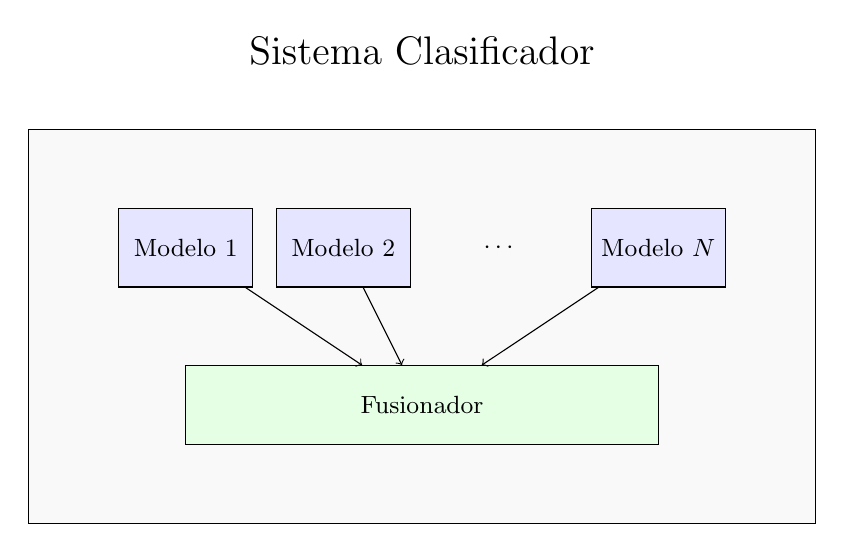
\begin{tikzpicture}[
    every node/.style={font=\small},
    modelo/.style={draw, fill=blue!10, minimum width=1.7cm, minimum height=1cm},
    fusionador/.style={draw, fill=green!10, minimum width=6cm, minimum height=1cm},
    sistema/.style={draw, fill=gray!5}
]
% Sistema
\node[sistema, minimum width=10cm, minimum height=5cm] (sistema) at (0,0) {};
\node[font=\Large] (titulo) at (0,3.5) {Sistema Clasificador};
% Modelos
\node[modelo] (modelo1) at (-3,1) {Modelo 1};
\node[modelo] (modelo2) at (-1,1) {Modelo 2};
\node at (1,1) {$\cdots$};
\node[modelo] (modeloN) at (3,1) {Modelo $N$};
% Fusionador
\node[fusionador] (fusionador) at (0,-1) {Fusionador};
% Aristas
\draw[->] (modelo1) to (fusionador);
\draw[->] (modelo2) to (fusionador);
\draw[->] (modeloN) to (fusionador);
\end{tikzpicture}
\end{center}
\end{frame}



\begin{frame}
\frametitle{Sistema ejemplo}
\begin{center}
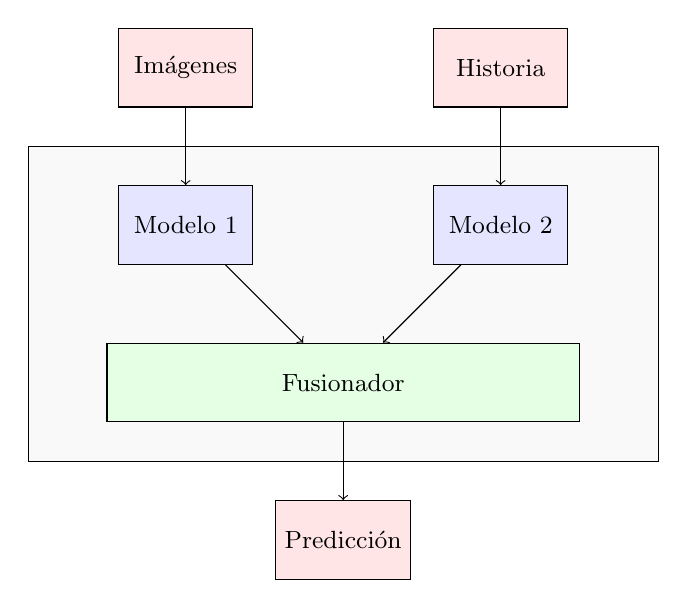
\begin{tikzpicture}[
every node/.style={font=\small},
datos/.style={draw, fill=red!10, minimum width=1.7cm, minimum height=1cm},
modelo/.style={draw, fill=blue!10, minimum width=1.7cm, minimum height=1cm},
fusionador/.style={draw, fill=green!10, minimum width=6cm, minimum height=1cm},
sistema/.style={draw, fill=gray!5}
]
% Datos
\node[datos] (datos1) at (-2,3) {Im\'agenes};
\node[datos] (datos2) at (2,3) {Historia};
% Sistema
\node[sistema, minimum width=8cm, minimum height=4cm] (sistema) at (0,0) {};
% Modelos
\node[modelo] (modelo1) at (-2,1) {Modelo 1};
\node[modelo] (modelo2) at (2,1) {Modelo 2};
% Fusionador
\node[fusionador] (fusionador) at (0,-1) {Fusionador};
% Salida
\node[datos] (resultado) at (0,-3) {Predicci\'on};
% Aristas
\draw[->] (datos1) to (modelo1);
\draw[->] (datos2) to (modelo2);
\draw[->] (modelo1) to (fusionador);
\draw[->] (modelo2) to (fusionador);
\draw[->] (fusionador) to (resultado);
\end{tikzpicture}
\end{center}
\end{frame}



\begin{frame}
\frametitle{Objetivo}
\begin{itemize}
\item Evaluar un modelo de forma independiente al sistema
\item Obtener una estimaci\'on \'util del comportamiento que tendr\'a el sistema con ese modelo
\end{itemize}
\end{frame}



\begin{frame}
\frametitle{Objetivo}
\begin{center}
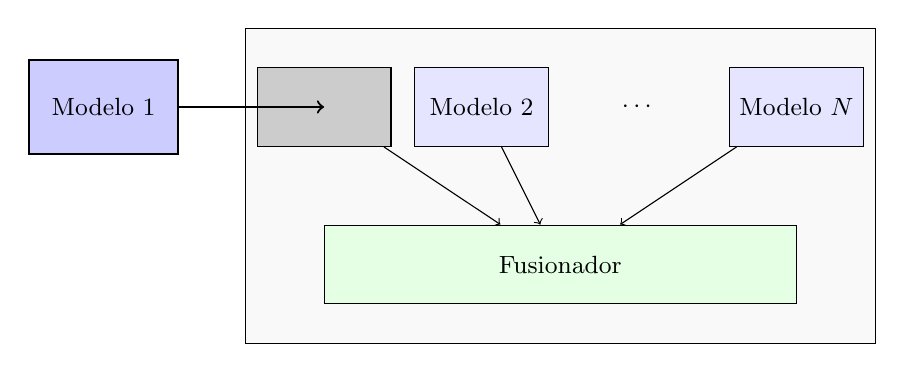
\begin{tikzpicture}[
    every node/.style={font=\small},
    modelo/.style={draw, fill=blue!10, minimum width=1.7cm, minimum height=1cm},
    fusionador/.style={draw, fill=green!10, minimum width=6cm, minimum height=1cm},
    sistema/.style={draw, fill=gray!5}
]
% Modelo externo
\node[modelo, fill=blue!20, thick, minimum width=1.9cm, minimum height=1.2cm] (modeloEvaluar) at (-5.8,1) {Modelo 1};
% Sistema
\node[sistema, minimum width=8cm, minimum height=4cm] (sistema) at (0,0) {};
% Modelos
\node[modelo, fill=gray!40] (modelo1) at (-3,1) {};
\node[modelo] (modelo2) at (-1,1) {Modelo 2};
\node at (1,1) {$\cdots$};
\node[modelo] (modeloN) at (3,1) {Modelo $N$};
% Fusionador
\node[fusionador] (fusionador) at (0,-1) {Fusionador};
% Aristas
\draw[->] (modelo1) to (fusionador);
\draw[->] (modelo2) to (fusionador);
\draw[->] (modeloN) to (fusionador);
\draw[->, thick]  (modeloEvaluar) to (-3,1);
\end{tikzpicture}
\end{center}
\end{frame}



\begin{frame}
\frametitle{Informaci\'on disponible}
Datos de los que se dispone para el problema:\\
\vspace{3mm}
\begin{itemize}
\item El sistema incompleto, faltando un modelo
\item Una funci\'on de costo para el sistema
\item Datos para la evaluaci\'on del sistema
\item El modelo a evaluar
\item Datos para la evaluaci\'on del modelo
\end{itemize}
\end{frame}



\begin{frame}
\frametitle{Informaci\'on disponible}
\begin{itemize}
\item Ambos conjuntos de datos pueden o no ser el mismo.
\item La funci\'on de costo del modelo es la que se busca proponer, y es dependiente de la funci\'on de costo del sistema y de la influencia del modelo en el sistema.
\end{itemize}
\end{frame}



\begin{frame}
\frametitle{Motivaci\'on}
Una posible utilidad de una funci\'on de costo para el modelo que sea independiente del sistema puede ser realizar b\'usqueda de hiperpar\'ametros. \\
\vspace{3mm}
Se puede querer reemplazar o añadir un modelo al sistema. Al momento de realizar la b\'usqueda de hiperpar\'ametros en el modelo, con un costo para el modelo independiente al sistema se puede comparar entre modelos de forma mucho mas r\'apida y asi elegir a los m\'as adecuados.
\end{frame}



% \begin{frame}
% \frametitle{Redes Bayesianas}
% La forma que se va a utilizar para modelar el problema es mediante una red bayesiana causal. Una red bayesiana causal es un DAG que se usa para representar distribuci\'ones probabilisticas sobre variables no independientes. Se tienen nodos para representar entidades, y aristas que representan causalidad entre esas entidades. Los nodos con doble c\'irculo son determin\'isticos dados los padres.
% \end{frame}



% \begin{frame}
% \frametitle{Redes Bayesianas}
% \centering
% \begin{tikzpicture}[scale=0.7, every node/.style={font=\tiny}]
% % Nodos
% \node[draw, fill=blue!30, minimum width=4.2cm, minimum height=3.3cm] at (0,5) (Sistema) {}; 
% \node[latent, font=\tiny, fill=green!10] at (0,10) (Persona) {$Persona$};
% \node[latent, double, font=\tiny, fill=green!40] at (3.5,8.5) (Clase) {$Clase$};
% \node[latent, font=\tiny, fill=green!10] at (-1,8) (Imagen) {$Imagen$};
% \node[latent, font=\tiny, fill=green!10] at (1,8) (Historia) {$Historia$};
% \node[latent, font=\tiny, fill=blue!20] at (-1,6) (Pred M1) {$Pred^{M1}$};
% \node[latent, font=\tiny, fill=blue!20] at (1,6) (Pred M2) {$Pred^{M2}$};
% \node[latent, double, font=\tiny, fill=blue!10] at (-2,4) (Conf M1) {$Conf^{M1}$};
% \node[latent, double, font=\tiny, fill=blue!10] at (2,4) (Conf M2) {$Conf^{M2}$};
% \node[latent, font=\tiny, fill=red!20] at (0,2) (Pred S) {$Pred^S$};
% \node[latent, double, font=\tiny, fill=red!10] at (0,0) (Conf S) {$Conf^S$};
% \node at (0,3.5) (Fusionador) {\textbf{fusionador}};
% \node[font=\large] at (-5.5,5) (Descripcion Sistema) {\color{blue} \underline{Sistema}};
% % Aristas
% \draw[->] (Persona) to (Clase);
% \draw[->] (Persona) to (Imagen);
% \draw[->] (Persona) to (Historia);
% \draw[->] (Imagen) to node[left] {\textbf{modelo 1}} (Pred M1);
% \draw[->] (Historia) to node[right] {\textbf{modelo 2}} (Pred M2);
% \draw[->] (Pred M1) to (Conf M1);
% \draw[->] (Pred M2) to (Conf M2);
% \draw[->] (Pred M1) to (Pred S);
% \draw[->] (Pred M2) to (Pred S);
% \draw[->] (Pred S) to (Conf S);
% \draw[->] (Clase) to[bend left] (Conf M1.east);
% \draw[->] (Clase.280) to[bend left] (Conf M2.north east);
% \draw[->] (Clase.south east) to[bend left] (Conf S.east);
% \draw[->, very thick, fill=blue, draw=blue] (Descripcion Sistema.east) to (Sistema.west);
% \end{tikzpicture}
% \end{frame}



\begin{frame}
\frametitle{Intervenci\'on}
Se va a utilizar una operaci\'on sobre el sistema llamada intervenci\'on, basada en la intervenci\'on de las redes bayesianas. \\
\vspace{3mm}
Al sistema sin el modelo se le inserta en ese lugar un modelo simple que hace siempre lo mismo a pesar del dato de entrada para poder analizar su comportamiento. \\
\end{frame}



\begin{frame}
\frametitle{Intervenci\'on}
Un ejemplo de intervenci\'on podr\'ia ser correr el sistema diciendole que el modelo devuelve siempre Positive. Luego se podr\'ia calcular la matriz de confusi\'on asociada a sus resultados. \\
\vspace{3mm}
La otra intervenci\'on que se va a usar es siempre Negative.
\end{frame}




% \begin{frame}
% \frametitle{Intervenci\'on}
% Un ejemplo del operador \textbf{do}:\\
% \vspace{3mm}
% \begin{minipage}{0.55\textwidth}
% \begin{itemize}
% \item $P(Y=y | X=x)$
% \item $P(Y=y | do(X=x))$
% \end{itemize}
% \end{minipage}
% \begin{minipage}{0.2\textwidth}
% \begin{center}
% \begin{tikzpicture}
% \node[latent] at (0,0.75) (nodeX) {$X$};
% \node[latent] at (0,-0.75) (nodeY) {$Y$};
% \draw[->] (nodeX) to (nodeY);
% \end{tikzpicture}
% \end{center}
% \end{minipage}
% \vspace{6mm}\\
% La consulta sin \textbf{do} es un condicional normal, donde miramos la probabilidad de $Y=y$ solo para los casos en los que $X=x$.\\
% \vspace{1mm}
% La consulta con el operador \textbf{do} se realiza sobre toda la distribuci\'on, asumiendo que $X$ vale $x$ siempre. 
% \end{frame}



\begin{frame}
\frametitle{Estimaci\'on del costo del sistema}
Para poder comparar entre modelos se separa el proceso en dos partes:\\
\vspace{3mm}
\begin{itemize}
\item Primero es evaluado el sistema sin el modelo, usando la intervenci\'on. Se registran las probabilidades de acierto en el sistema intervenido con un modelo que da siempre positive, y uno que da siempre negative.
\item Luego usando esos valores, se ejecuta el modelo de forma independiente para calcular alguna funci\'on de costo asociada.
\end{itemize}
\end{frame}



\begin{frame}
\frametitle{Estimaci\'on del costo del sistema}
\begin{itemize}
\item Idealmente, se buscar\'ia estimar de forma precisa el resultado de la ejecuci\'on del sistema si se hubiera corrido con el modelo. 
\item Esto es imposible ya que dados modelos distintos la misma matriz de confusi\'on pueden llevar a resultados muy distintos en el sistema segun su predicci\'on en cada instancia.
\item Por lo tanto la m\'etrica a evaluar va a ser, dado un sistema y dada la matriz de confusi\'on de un modelo, estimar el peor caso del sistema ejecutado con ese modelo. 
\end{itemize}
\end{frame}
\begin{frame}[t]
\frametitle{Notaci\'on}
\vspace{6mm}
Para definir el problema formalmente se introduce la notaci\'on $m^{f,D}_{ij}$ para denotar un valor de una matriz de confusi\'on: \\
\vspace{3mm}
$m^{f,D}_{ij}$ = $|$$\{d \in D $ $|$ $f(d_{1})=i \land d_{2}=j\}$$|$ \\
\vspace{3mm}
\begin{itemize}
\item $i$ es la clase real
\item $j$ es la clase que predice el modelo f sobre el dato
\item $D$ es el dataset utilizado, conteniendo un conjunto de pares $d_1$ instancia, $d_2$ clase real y su valor por defecto que representa todos los datos disponibles es $D$
\item $f$ es el modelo usado y puede valer:\\
\begin{itemize}
\item $M$ como el modelo a analizar\\
\item $S$ como el sistema completo con el modelo\\
\item $S_{M=X}$ como el sistema con un modelo intervenido que predice siempre la clase $X$ para cualquier instancia\\
\end{itemize}
\end{itemize}
\end{frame}



\begin{frame}[t]
\frametitle{Especificaci\'on del problema}
\vspace{6mm}
Se espera lo siguiente sobre el comportamiento del sistema:\\
\vspace{4mm}

\begin{itemize}

\item {$\{d\in D$ $|$ $ d_{2}=0 \land S(d_{1})=0 \land M(d_{1})=1\}$ $\subseteq$

$\{d\in D$ $|$ $ d_{2}=0 \land S(d_{1})=0 \land M(d_{1})=0\}$}
% \vspace{2mm}
% \item {$\{d\in D$ $|$ $ d_{2}=0 \land S(d_{1})=1 \land M(d_{1})=0\}$ $\subseteq$

% $\{d\in D$ $|$ $ d_{2}=0 \land S(d_{1})=1 \land M(d_{1})=1\}$}
% \vspace{2mm}
% \item {$\{d\in D$ $|$ $ d_{2}=1 \land S(d_{1})=1 \land M(d_{1})=0\}$ $\subseteq$

% $\{d\in D$ $|$ $ d_{2}=1 \land S(d_{1})=1 \land M(d_{1})=1\}$}
% \vspace{2mm}
% \item {$\{d\in D$ $|$ $ d_{2}=1 \land S(d_{1})=0 \land M(d_{1})=1\}$ $\subseteq$

% $\{d\in D$ $|$ $ d_{2}=1 \land S(d_{1})=0 \land M(d_{1})=0\}$}
\end{itemize}
\vspace{4mm}
$\symbol{92}$$\symbol{92}$ Agregar evidencia solo puede mejorar la predicci\'on
\end{frame}



\begin{frame}[t]
\frametitle{Especificaci\'on del problema}
\vspace{6mm}
Se espera lo siguiente sobre el comportamiento del sistema:\\
\vspace{4mm}

\begin{itemize}

% \item {$\{d\in D$ $|$ $ d_{2}=0 \land S(d_{1})=0 \land M(d_{1})=1\}$ $\subseteq$

% $\{d\in D$ $|$ $ d_{2}=0 \land S(d_{1})=0 \land M(d_{1})=0\}$}
\vspace{12.5mm}
\item {$\{d\in D$ $|$ $ d_{2}=0 \land S(d_{1})=1 \land M(d_{1})=0\}$ $\subseteq$

$\{d\in D$ $|$ $ d_{2}=0 \land S(d_{1})=1 \land M(d_{1})=1\}$}
% \vspace{2mm}
% \item {$\{d\in D$ $|$ $ d_{2}=1 \land S(d_{1})=1 \land M(d_{1})=0\}$ $\subseteq$

% $\{d\in D$ $|$ $ d_{2}=1 \land S(d_{1})=1 \land M(d_{1})=1\}$}
% \vspace{2mm}
% \item {$\{d\in D$ $|$ $ d_{2}=1 \land S(d_{1})=0 \land M(d_{1})=1\}$ $\subseteq$

% $\{d\in D$ $|$ $ d_{2}=1 \land S(d_{1})=0 \land M(d_{1})=0\}$}
\end{itemize}
\vspace{4mm}
$\symbol{92}$$\symbol{92}$ Restar evidencia solo puede empeorar la predicci\'on
\end{frame}



\begin{frame}[t]
\frametitle{AssEspecificaci\'on del problemaumptions}
\vspace{6mm}
Se espera lo siguiente sobre el comportamiento del sistema:\\
\vspace{4mm}

\begin{itemize}

\item {$\{d\in D$ $|$ $ d_{2}=0 \land S(d_{1})=0 \land M(d_{1})=1\}$ $\subseteq$

$\{d\in D$ $|$ $ d_{2}=0 \land S(d_{1})=0 \land M(d_{1})=0\}$}
\vspace{2mm}
\item {$\{d\in D$ $|$ $ d_{2}=0 \land S(d_{1})=1 \land M(d_{1})=0\}$ $\subseteq$

$\{d\in D$ $|$ $ d_{2}=0 \land S(d_{1})=1 \land M(d_{1})=1\}$}
\vspace{2mm}
\item {$\{d\in D$ $|$ $ d_{2}=1 \land S(d_{1})=1 \land M(d_{1})=0\}$ $\subseteq$

$\{d\in D$ $|$ $ d_{2}=1 \land S(d_{1})=1 \land M(d_{1})=1\}$}
\vspace{2mm}
\item {$\{d\in D$ $|$ $ d_{2}=1 \land S(d_{1})=0 \land M(d_{1})=1\}$ $\subseteq$

$\{d\in D$ $|$ $ d_{2}=1 \land S(d_{1})=0 \land M(d_{1})=0\}$}
\end{itemize}
\vspace{4mm}
$\symbol{92}$$\symbol{92}$ Lo mismso para Clase Negative
\end{frame}



\begin{frame}
\frametitle{Especificaci\'on del problema}
Se espera lo siguiente sobre la funci\'on de costo asociada a las confusiones del sistema:\\
\vspace{4mm}
\begin{itemize}
\item \SCTP $\leq$ \SCFN \\
\vspace{2mm}
\item \SCTN $\leq$ \SCFP \\
\end{itemize}
\vspace{4mm}
Los fallos tienen mayor costo que los aciertos.
\end{frame}



\begin{frame}
\frametitle{Especificaci\'on del problema}
Datos disponibles:
\begin{table}[]
    \begin{minipage}{0.62\textwidth}
        \begin{tabular}{c|c|c|}
            & Pred Pos & Pred Neg \\ \hline
            Clase Pos & \IPTP & \IPFN \\ \hline
            Clase Neg & \IPFP & \IPTN \\ \hline
        \end{tabular}
    \end{minipage}
    \begin{minipage}{0.34\textwidth}
        \caption{Matriz de confusi\'on del sistema si Modelo = Positive}
    \end{minipage}
\end{table}
\begin{table}[]
    \begin{minipage}{0.62\textwidth}
        \begin{tabular}{c|c|c|}
            & Pred Pos & Pred Neg \\ \hline
            Clase Pos & \INTP & \INFN \\ \hline
            Clase Neg & \INFP & \INTN \\ \hline
        \end{tabular}
    \end{minipage}
    \begin{minipage}{0.34\textwidth}
        \caption{Matriz de confusi\'on del sistema si Modelo = Negative}
    \end{minipage}
\end{table}
\end{frame}



\begin{frame}
\frametitle{Especificaci\'on del problema}
Otros datos disponibles: \\
\vspace{3mm}
\begin{table}[]
    \begin{minipage}{0.60\textwidth}
        \begin{tabular}{c|c|c|}
            & Positive & Negative \\ \hline
            \#Instancias & P & N \\ \hline
        \end{tabular}
    \end{minipage}
    \begin{minipage}{0.38\textwidth}
        \caption{Cantidad de instancias por clase}
    \end{minipage}
\end{table}
\begin{table}[]
    \begin{minipage}{0.60\textwidth}
        \begin{tabular}{c|c|c|}
            & Pred Pos & Pred Neg \\ \hline
            Clase Pos & \MTP & \MFN \\ \hline
            Clase Neg & \MFP & \MTN \\ \hline
        \end{tabular}
    \end{minipage}
    \begin{minipage}{0.38\textwidth}
        \caption{Matriz de confusi\'on del modelo}
    \end{minipage}
\end{table}
\end{frame}



\begin{frame}
\frametitle{Especificaci\'on del problema}
Dados esos datos, se busca generar la peor matriz de confusi\'on posible del sistema que sea v\'alida (peor caso).
\vspace{3mm}
\begin{table}[]
    \begin{tabular}{c|c|c|}
        & Prediccion Positive & Prediccion Negative \\ \hline
        Clase Positive & \STP & \SFN \\ \hline
        Clase Negative & \SFP & \STN \\ \hline
    \end{tabular}
    \caption{Matriz de confusi\'on del sistema}
\end{table}
\end{frame}



\begin{frame}
\frametitle{Especificaci\'on del problema}
La peor es la que maximiza: \\
\vspace{3mm}
\begin{itemize}
\item {$\STP$ * $\SCTP$ + $\SFN$ * $\SCFN$ + 

$\SFP$ * $\SCFP$ + $\STN$ * $\SCTN$}
\end{itemize}
\vspace{3mm}
Como los costos asociados a las confusiones de aciertos son menores a las de fallos, es equivalente a maximizar: \\
\vspace{3mm}
\begin{itemize}
\item $\SFN$ + $\SFP$
\end{itemize}
\end{frame}



\begin{frame}
\frametitle{Cotas independientes al modelo}
Si se logra acotar de forma exacta las confusiones del sistema, particularmente hallar una cota superior para $\SFN$ y $\SFP$, podemos tomar ese valor m\'aximo como el valor de la confusi\'on en peor caso. \\
\vspace{3mm}
Para las confusiones restantes $\STP$ y $\STN$ se toman las instancias restantes de la clase que deberian correspoonder a su cota inferior.
\end{frame}




\begin{frame}[t]
\frametitle{Cotas independientes al modelo}
\vspace{6mm}
Cotas a las confusiones del sistema (independientes al modelo): \\
\vspace{6mm}
\begin{minipage}[t]{0.5\textwidth}
\begin{itemize}
  \setcounter{enumi}{0}
  \item \STP + \SFN = P
  \item \STN + \SFP = N
\end{itemize}
\end{minipage}
\begin{minipage}[t]{0.46\textwidth}
\vspace{2mm}
$\symbol{92}$$\symbol{92}$ Total de instancias por clase
\end{minipage}
\end{frame}



\begin{frame}[t]
\frametitle{Cotas independientes al modelo}
\vspace{6mm}
Cotas a las confusiones del sistema (independientes al modelo): \\
\vspace{6mm}
\begin{minipage}[t]{0.5\textwidth}
\begin{itemize}
  \setcounter{enumi}{0}
  \item \STP + \SFN = P
  \item \STN + \SFP = N
  \vspace{3mm}
  \item \INTP $\leq$ \STP $\leq$ \IPTP
\end{itemize}
\end{minipage}
\begin{minipage}[t]{0.46\textwidth}
\vspace{15mm}
$\symbol{92}$$\symbol{92}$ M\'as aciertos que cuando el modelo falla siempre, menos aciertos que cuando el modelo acierta siempre
\end{minipage}
\end{frame}



\begin{frame}[t]
\frametitle{Cotas independientes al modelo}
\vspace{6mm}
Cotas a las confusiones del sistema (independientes al modelo): \\
\vspace{6mm}
\begin{minipage}[t]{0.5\textwidth}
\begin{itemize}
  \setcounter{enumi}{0}
  \item \STP + \SFN = P
  \item \STN + \SFP = N
  \vspace{3mm}
  \item \INTP $\leq$ \STP $\leq$ \IPTP
  \item \IPFN $\leq$ \SFN $\leq$ \INFN
\end{itemize}
\end{minipage}
\begin{minipage}[t]{0.46\textwidth}
\vspace{24mm}
$\symbol{92}$$\symbol{92}$ M\'as fallos que cuando el modelo acierta siempre, menos fallos que cuando el modelo falla siempre
\end{minipage}
\end{frame}



\begin{frame}[t]
\frametitle{Cotas independientes al modelo}
\vspace{6mm}
Cotas a las confusiones del sistema (independientes al modelo): \\
\vspace{6mm}
\begin{minipage}[t]{0.5\textwidth}
\begin{itemize}
  \setcounter{enumi}{0}
  \item \STP + \SFN = P
  \item \STN + \SFP = N
  \vspace{3mm}
  \item \INTP $\leq$ \STP $\leq$ \IPTP
  \item \IPFN $\leq$ \SFN $\leq$ \INFN
  \vspace{3mm}
  \item \INFP $\leq$ \SFP $\leq$ \IPFP
  \item \IPTN $\leq$ \STN $\leq$ \INTN
\end{itemize}
\end{minipage}
\begin{minipage}[t]{0.46\textwidth}
\vspace{30mm}
$\symbol{92}$$\symbol{92}$ Lo mismo para la clase Negative
\end{minipage}
\end{frame}



\begin{frame}
\frametitle{Cotas independientes al modelo}
Hasta ahora se tienen unos valores que acotan superior e inferiormente a cada confusi\'on del sistema. Este rango es independiente del modelo y potencialmente muy laxo. \\
\vspace{3mm}
A continuacion se va a analizar de forma m\'as cercana los posibles resultados de las instancias en base a lo que se sabe del modelo y del comportamiento del sistema para poder acotar de forma m\'as ajustada. 
\end{frame}
\begin{frame}
\frametitle{An\'alisis de peor caso}
La siguiente tabla tiene para con conjunto de instancias de ejemplo de clase Positive, que resultado tendr\'ia el sistema en caso del modelo predecir Positive o Negative. \\
\vspace{3mm}
Se marca con una X las instancias donde el sistema falla. La suma de la cantidad de X por columna son los valores con intervenci\'on mencionados anteriormente en \IPFN y \INFN. Se busca ilustrar que casos no son v\'alidos en base a las assumptions planteadas.\\
\vspace{3mm}
El mismo an\'alisis es v\'alido para la clase Negative.
\end{frame}



\newcommand{\CIP}{\text{$m^{S^{M=P},i}_{01}$}}
\newcommand{\CIN}{\text{$m^{S^{M=N},i}_{01}$}}
\newcommand{\CS}{\text{$m^{S,i}_{01}$}}
\begin{frame}
\frametitle{An\'alisis de peor caso}
Recordando la assumption 2 de la clase Positive:\\
\vspace{3mm}
{$\{d\in D$ $|$ $ d_{2}=0 \land S(d_{1})=0 \land M(d_{1})=1\}$ $\subseteq$

$\{d\in D$ $|$ $ d_{2}=0 \land S(d_{1})=0 \land M(d_{1})=0\}$}
\vspace{3mm}
\begin{table}[]
    \begin{tabular}{c|c|c|c|}
        & \CIP & \CIN & Es V\'alido \\ \hline
                            Instancia 1 &   &   &    \\ \hline
                            Instancia 2 & X &   &    \\ \hline
                            Instancia 3 &   & X &    \\ \hline
                            Instancia 4 & X & X &    \\ \hline
    \end{tabular}
    \caption{Resultados posibles en instancias de clase Positive}
\end{table}
\end{frame}



\begin{frame}
\frametitle{An\'alisis de peor caso}
Recordando la assumption 2 de la clase Positive:\\
\vspace{3mm}
{$\{d\in D$ $|$ $ d_{2}=0 \land S(d_{1})=0 \land M(d_{1})=1\}$ $\subseteq$

$\{d\in D$ $|$ $ d_{2}=0 \land S(d_{1})=0 \land M(d_{1})=0\}$}
\vspace{3mm}
\begin{table}[]
    \begin{tabular}{c|c|c|c|}
        & \CIP & \CIN & Es V\'alido \\ \hline
        \rowcolor{green!30} Instancia 1 &   &   & SI \\ \hline
                            Instancia 2 & X &   &    \\ \hline
                            Instancia 3 &   & X &    \\ \hline
                            Instancia 4 & X & X &    \\ \hline
    \end{tabular}
    \caption{Resultados posibles en instancias de clase Positive}
\end{table}
\end{frame}



\begin{frame}
\frametitle{An\'alisis de peor caso}
Recordando la assumption 2 de la clase Positive:\\
\vspace{3mm}
{$\{d\in D$ $|$ $ d_{2}=0 \land S(d_{1})=0 \land M(d_{1})=1\}$ $\subseteq$

$\{d\in D$ $|$ $ d_{2}=0 \land S(d_{1})=0 \land M(d_{1})=0\}$}
\vspace{3mm}
\begin{table}[]
    \begin{tabular}{c|c|c|c|}
        & \CIP & \CIN & Es V\'alido \\ \hline
                            Instancia 1 &   &   & SI \\ \hline
        \rowcolor{red!30}   Instancia 2 & X &   & NO \\ \hline
                            Instancia 3 &   & X &    \\ \hline
                            Instancia 4 & X & X &    \\ \hline
    \end{tabular}
    \caption{Resultados posibles en instancias de clase Positive}
\end{table}
\end{frame}



\begin{frame}
\frametitle{An\'alisis de peor caso}
Recordando la assumption 2 de la clase Positive:\\
\vspace{3mm}
{$\{d\in D$ $|$ $ d_{2}=0 \land S(d_{1})=0 \land M(d_{1})=1\}$ $\subseteq$

$\{d\in D$ $|$ $ d_{2}=0 \land S(d_{1})=0 \land M(d_{1})=0\}$}
\vspace{3mm}
\begin{table}[]
    \begin{tabular}{c|c|c|c|}
        & \CIP & \CIN & Es V\'alido \\ \hline
                            Instancia 1 &   &   & SI \\ \hline
                            Instancia 2 & X &   & NO \\ \hline
        \rowcolor{green!30} Instancia 3 &   & X & SI \\ \hline
                            Instancia 4 & X & X &    \\ \hline
    \end{tabular}
    \caption{Resultados posibles en instancias de clase Positive}
\end{table}
\end{frame}



\begin{frame}
\frametitle{An\'alisis de peor caso}
Recordando la assumption 2 de la clase Positive:\\
\vspace{3mm}
{$\{d\in D$ $|$ $ d_{2}=0 \land S(d_{1})=0 \land M(d_{1})=1\}$ $\subseteq$

$\{d\in D$ $|$ $ d_{2}=0 \land S(d_{1})=0 \land M(d_{1})=0\}$}
\vspace{3mm}
\begin{table}[]
    \begin{tabular}{c|c|c|c|}
        & \CIP & \CIN & Es V\'alido \\ \hline
                            Instancia 1 &   &   & SI \\ \hline
                            Instancia 2 & X &   & NO \\ \hline
                            Instancia 3 &   & X & SI \\ \hline
        \rowcolor{green!30} Instancia 4 & X & X & SI \\ \hline
    \end{tabular}
    \caption{Resultados posibles en instancias de clase Positive}
\end{table}
\end{frame}



\begin{frame}
\frametitle{An\'alisis de peor caso}
Ahora sabiendo de que formas se pueden comportar las instancias, se observar\'an distintas posibles combinaci\'ones de  confusiones del sistema para las instancias de clase Positive, fijando los resultados del modelo. Si una fila es verde el modelo predice Positive y si es roja predice Negative. Al fijar el modelo se fijan la cantidad de predicci\'ones Positive y Negative, pero hay muchas formas de adquirir la misma confusi\'on que llevan a distintas confusiones del sistema.\\
\vspace{3mm}
La cantidad total de X en la columna de Positive es \IPFN y la cantidad total de X en la columna de Negative es \INFN.\\
\end{frame}



% \newcolumntype{C}[1]{>{\centering\arraybackslash}p{#1}}
% \begin{frame}
% \frametitle{An\'alisis de peor caso}
% \begin{table}[t]
%     \begin{tabular}{c|C{1.5cm}|C{1.5cm}|C{1.5cm}|}
%         & \CIP & \CIN & \CS \\ \hline
%         \rowcolor{green!25} Instancia 1 & \cellcolor{green!50}   & X & TP \\ \hline
%         \rowcolor{green!25} Instancia 2 & \cellcolor{green!50}   & X & TP \\ \hline
%         \rowcolor{green!25} Instancia 3 & \cellcolor{green!50}   &   & TP \\ \hline
%         \rowcolor{green!25} Instancia 4 & \cellcolor{green!50} X & X & FN \\ \hline
%         \rowcolor{red!25}   Instancia 5 &   & \cellcolor{red!50}     & TP \\ \hline
%         \rowcolor{red!25}   Instancia 6 &   & \cellcolor{red!50}   X & FN \\ \hline
%         \rowcolor{red!25}   Instancia 7 &   & \cellcolor{red!50}   X & FN \\ \hline
%         \rowcolor{red!25}   Instancia 8 &   & \cellcolor{red!50}   X & FN \\ \hline
%     \end{tabular}
%     \caption{Ejemplo Clase Positive 1}
% \end{table}
% \vspace{3mm}
% \centering{Cantidad de True Positives totales: 4}\\
% \centering{Cantidad de False Negatives totales: 4}\\
% \end{frame}



% \begin{frame}
% \frametitle{An\'alisis de peor caso}
% \begin{table}[]
%     \begin{tabular}{c|C{1.5cm}|C{1.5cm}|C{1.5cm}|}
%         & \CIP & \CIN & \CS \\ \hline
%         \rowcolor{green!25} Instancia 1 & \cellcolor{green!50}   & X & TP \\ \hline
%         \rowcolor{green!25} Instancia 2 & \cellcolor{green!50}   & X & TP \\ \hline
%         \rowcolor{red!25}   Instancia 3 &   & \cellcolor{red!50}     & TP \\ \hline
%         \rowcolor{red!25}   Instancia 4 & X & \cellcolor{red!50}   X & FN \\ \hline
%         \rowcolor{red!25}   Instancia 5 &   & \cellcolor{red!50}   X & FN \\ \hline
%         \rowcolor{green!25} Instancia 6 & \cellcolor{green!50}   &   & TP \\ \hline
%         \rowcolor{green!25} Instancia 7 & \cellcolor{green!50}   & X & TP \\ \hline
%         \rowcolor{red!25}   Instancia 8 &   & \cellcolor{red!50}   X & FN     \\ \hline
%     \end{tabular}
%     \caption{Ejemplo Clase Positive 2}
% \end{table}
% \vspace{3mm}
% \centering{Cantidad de True Positives totales: 5}\\
% \centering{Cantidad de False Negatives totales: 3}\\
% \end{frame}



% \begin{frame}
% \frametitle{An\'alisis de peor caso}
% \begin{table}[t]
%     \begin{tabular}{c|C{1.5cm}|C{1.5cm}|C{1.5cm}|}
%         & \CIP & \CIN & \CS \\ \hline
%         \rowcolor{red!25}   Instancia 1 &   & \cellcolor{red!50}   X & FN \\ \hline
%         \rowcolor{green!25} Instancia 2 & \cellcolor{green!50}   & X & TP \\ \hline
%         \rowcolor{green!25} Instancia 3 & \cellcolor{green!50}   &   & TP \\ \hline
%         \rowcolor{green!25} Instancia 4 & \cellcolor{green!50} X & X & FN \\ \hline
%         \rowcolor{green!25} Instancia 5 & \cellcolor{green!50}   &   & TP \\ \hline
%         \rowcolor{red!25}   Instancia 6 &   & \cellcolor{red!50}   X & FN \\ \hline
%         \rowcolor{red!25}   Instancia 7 &   & \cellcolor{red!50}   X & FN \\ \hline
%         \rowcolor{red!25}   Instancia 8 &   & \cellcolor{red!50}   X & FN \\ \hline
%     \end{tabular}
%     \caption{Ejemplo Clase Positive 3}
% \end{table}
% \vspace{3mm}
% \centering{Cantidad de True Positives totales: 3}\\
% \centering{Cantidad de False Negatives totales: 5}\\
% \end{frame}



\newcolumntype{C}[1]{>{\centering\arraybackslash}p{#1}}
\begin{frame}
\frametitle{An\'alisis de peor caso}
\begin{table}[t]
    \begin{tabular}{c|C{1.5cm}|C{1.5cm}|C{1.5cm}|}
        & \CIP & \CIN & \CS \\ \hline
        \rowcolor{green!25} Instancia 1 & \cellcolor{green!50}   & X & \cellcolor{green!50}   \\ \hline
        \rowcolor{green!25} Instancia 2 & \cellcolor{green!50}   & X & \cellcolor{green!50}   \\ \hline
        \rowcolor{green!25} Instancia 3 & \cellcolor{green!50}   &   & \cellcolor{green!50}   \\ \hline
        \rowcolor{green!25} Instancia 4 & \cellcolor{green!50} X & X & \cellcolor{green!50} X \\ \hline
        \rowcolor{red!25}   Instancia 5 &   & \cellcolor{red!50}     & \cellcolor{red!50}   \\ \hline
        \rowcolor{red!25}   Instancia 6 &   & \cellcolor{red!50}   X & \cellcolor{red!50} X \\ \hline
        \rowcolor{red!25}   Instancia 7 &   & \cellcolor{red!50}   X & \cellcolor{red!50} X \\ \hline
        \rowcolor{red!25}   Instancia 8 &   & \cellcolor{red!50}   X & \cellcolor{red!50} X \\ \hline
    \end{tabular}
    \caption{Ejemplo Clase Positive 1}
\end{table}
\vspace{3mm}
\centering{Cantidad de True Positives totales: 4}\\
\centering{Cantidad de False Negatives totales: 4}\\
\end{frame}



\begin{frame}
\frametitle{An\'alisis de peor caso}
\begin{table}[]
    \begin{tabular}{c|C{1.5cm}|C{1.5cm}|C{1.5cm}|}
        & \CIP & \CIN & \CS \\ \hline
        \rowcolor{green!25} Instancia 1 & \cellcolor{green!50}   & X & \cellcolor{green!50}   \\ \hline
        \rowcolor{green!25} Instancia 2 & \cellcolor{green!50}   & X & \cellcolor{green!50}   \\ \hline
        \rowcolor{red!25}   Instancia 3 &   & \cellcolor{red!50}     & \cellcolor{red!50}   \\ \hline
        \rowcolor{red!25}   Instancia 4 & X & \cellcolor{red!50}   X & \cellcolor{red!50} X \\ \hline
        \rowcolor{red!25}   Instancia 5 &   & \cellcolor{red!50}   X & \cellcolor{red!50} X \\ \hline
        \rowcolor{green!25} Instancia 6 & \cellcolor{green!50}   &   & \cellcolor{green!50}   \\ \hline
        \rowcolor{green!25} Instancia 7 & \cellcolor{green!50}   & X & \cellcolor{green!50}   \\ \hline
        \rowcolor{red!25}   Instancia 8 &   & \cellcolor{red!50}   X & \cellcolor{red!50} X \\ \hline
    \end{tabular}
    \caption{Ejemplo Clase Positive 2}
\end{table}
\vspace{3mm}
\centering{Cantidad de True Positives totales: 5}\\
\centering{Cantidad de False Negatives totales: 3}\\
\end{frame}



\begin{frame}
\frametitle{An\'alisis de peor caso}
\begin{table}[t]
    \begin{tabular}{c|C{1.5cm}|C{1.5cm}|C{1.5cm}|}
        & \CIP & \CIN & \CS \\ \hline
        \rowcolor{red!25}   Instancia 1 &   & \cellcolor{red!50}   X & \cellcolor{red!50} X \\ \hline
        \rowcolor{green!25} Instancia 2 & \cellcolor{green!50}   & X & \cellcolor{green!50}   \\ \hline
        \rowcolor{green!25} Instancia 3 & \cellcolor{green!50}   &   & \cellcolor{green!50}   \\ \hline
        \rowcolor{green!25} Instancia 4 & \cellcolor{green!50} X & X & \cellcolor{green!50} X \\ \hline
        \rowcolor{green!25} Instancia 5 & \cellcolor{green!50}   &   & \cellcolor{green!50}   \\ \hline
        \rowcolor{red!25}   Instancia 6 &   & \cellcolor{red!50}   X & \cellcolor{red!50} X \\ \hline
        \rowcolor{red!25}   Instancia 7 &   & \cellcolor{red!50}   X & \cellcolor{red!50} X \\ \hline
        \rowcolor{red!25}   Instancia 8 &   & \cellcolor{red!50}   X & \cellcolor{red!50} X \\ \hline
    \end{tabular}
    \caption{Ejemplo Clase Positive 3}
\end{table}
\vspace{3mm}
\centering{Cantidad de True Positives totales: 3}\\
\centering{Cantidad de False Negatives totales: 5}\\
\end{frame}
\begin{frame}
\frametitle{An\'alisis de peor caso}
Se puede observar como para 3 modelos ejemplo con la misma matriz de confusi\'on, se obtienen 3 resultados de sistema distintos. La causa de esto son las instancias con una sola X, sobre las cuales si el modelo predice Positive, el resultado del sistema es un True Positive y si el modelo predice Positive, el resultado del sistema es un False Negative. \\
\vspace{3mm}
Ahora se busca saber cual es la cantidad de False Negatives m\'axima y la cantidad de True Positive m\'axima luego de fijar el modelo, y as\'i ajustar la cota anterior.\\
\end{frame}



\begin{frame}
\frametitle{An\'alisis de peor caso}
Las confusiones del sistema se pueden particionar de la siguiente manera: \\
\vspace{3mm}
\begin{itemize}
\item $\STP$ = $\STPMP$ + $\STPMN$ \\
\item $\SFN$ = $\SFNMP$ + $\SFNMN$ \\
\end{itemize}
\vspace{3mm}
Con el objetivo de separar en casos por resultado del modelo y acotar ambos casos por separado.
\end{frame}



\begin{frame}
\frametitle{An\'alisis de peor caso}
La cantidad m\'axima de False Negatives ocurre cuando: \\
\vspace{3mm}
\begin{itemize}
\item $\STPMP$ tiene la m\'axima cantidad de instancias con doble X posibles. \\
\item $\STPMN$ tiene la m\'axima cantidad de instancias con una X posibles. \\
\end{itemize}
\vspace{3mm}
De esta forma todas las instancias con una X que sea posible considerar como False Negatives del modelo van a serlo.
\end{frame}



\begin{frame}
\vspace{9mm}
\frametitle{An\'alisis de peor caso}
Escribiendo formalmente la cota superior de fallos para la clase Positive: \\
\vspace{6mm}
\begin{itemize}
\item $\SFNMP$ = Min(\MTP, \IPFN) \\
% \vspace{3mm}
% \item $\SFPMN$ = Min(\MTN, \INFP) \\
\vspace{3mm}
\item $\SFNMN$ = Min(\MFN, \INFN - Min(\MTP, \IPFN)) \\
% \vspace{3mm}
% \item $\SFPMP$ = Min(\MFP, \IPFP - Min(\MTN, \INFP)) \\
\end{itemize}
\end{frame}



\begin{frame}
\frametitle{An\'alisis de peor caso}
Definiendo la cota superior a los fallos del sistema, e inferior a los aciertos, dado que se saben las confusiones del modelo: \\
\vspace{6mm}
$\STP$ $\geq$ (\MTP - Min(\MTP, \IPFN)) + \\
\vspace{1mm}
\hspace{12.2mm}
(\MFN - Min(\MFN, \INFN - Min(\MTP, \IPFN))) \\
\vspace{2mm}
$\SFN$ $\leq$ Min(\MTP, \IPFN) + \\
\vspace{1mm}
\hspace{12.2mm}
Min(\MFN, \INFN - Min(\MTP, \IPFN)) \\
\end{frame}
\begin{frame}
\frametitle{An\'alisis de peor caso}
La cantidad m\'axima de True Positives ocurre cuando: \\
\vspace{3mm}
\begin{itemize}
\item \STPMP tiene la m\'axima cantidad de instancias con una X posibles. \\
\item \STPMN tiene la m\'axima cantidad de instancias con doble X posibles. \\
\end{itemize}
\vspace{3mm}
De esta forma todas las instancias con una X que sea posible considerar como True Positives del modelo van a serlo, evitando sus fallos en la clasificaci\'on.
\end{frame}



\begin{frame}
\frametitle{An\'alisis de peor caso}
Escribiendo formalmente la cota superior de aciertos para la clase
Positive: \\
\vspace{3mm}
\begin{itemize}
\item \STPMP = Min(\MTP, \IPTP - Min(\MFN, \INTP)) \\
% \vspace{3mm}
% \item $\STNMN$ = Min(\MTN, \INTN - Min(\MFP, \IPTN)) \\
\vspace{3mm}
\item \STPMN = Min(\MFN, \INTP) \\
% \vspace{3mm}
% \item $\STNFP$ = Min(\MFP, \IPTN) \\
\end{itemize}
\end{frame}



\begin{frame}
\frametitle{An\'alisis de peor caso}
Definiendo la cota superior a los aciertos del sistema, y superior a los aciertos, dado que se saben las confusiones del modelo: \\
\vspace{6mm}
$\STP$ $\leq$ Min(\MTP, \IPTP - Min(\MFN, \INTP)) + \\
\vspace{1mm}
\hspace{12.2mm}
Min(\MFN, \INTP) \\
\vspace{2mm}
$\SFN$ $\geq$ (\MTP - Min(\MTP, \IPTP - Min(\MFN, \INTP))) + \\
\vspace{1mm}
\hspace{12.2mm}
(\MFN - Min(\MFN, \INTP)) \\
\end{frame}



\begin{frame}
\frametitle{An\'alisis de peor caso}
A su vez, el mismo an\'alisis es v\'alido para la clase Negative, llegando a las siguientes cotas: \\
\vspace{3mm}
Cota superior a los fallos del sistema, e inferior a los aciertos, dado que se saben las confusiones del modelo: \\
\vspace{6mm}
$\SFP$ $\leq$ Min(\MTN, \INFP) + \\
\vspace{1mm}
\hspace{11mm}
Min(\MFP, \IPFP - Min(\MTN, \INFP)) \\
\vspace{2mm}
$\STN$ $\geq$ (\MTN - Min(\MTN, \INFP)) + \\
\vspace{1mm}
\hspace{11mm}
(\MFP - Min(\MFP, \IPFP - Min(\MTN, \INFP))) \\
\end{frame}



\begin{frame}
\frametitle{An\'alisis de peor caso}
Cota superior a los aciertos del sistema, e inferior a los fallos, dado que se saben las confusiones del modelo:\\
\vspace{6mm}
$\SFP$ $\geq$  (\MTN - Min(\MTN, \INTN - Min(\MFP, \IPTN))) + \\
\vspace{1mm}
\hspace{11mm}
(\MFP - Min(\MFP, \IPTN)) \\
\vspace{2mm}
$\STN$ $\leq$ Min(\MTN, \INTN - Min(\MFP, \IPTN)) + \\
\vspace{1mm}
\hspace{11mm}
Min(\MFP, \IPTN) \\
\end{frame}



\begin{frame}
\frametitle{An\'alisis de peor caso}
Como el objetivo es encontrar el m\'aximo para $\SFN$ y $\SFP$ se toma el valor de esas confusiones igual a sus cotas superiores, y las confusiones $\STP$ y $\STN$ asociadas iguales a sus cotas inferiores. \\
\end{frame}



\begin{frame}
\frametitle{An\'alisis de peor caso}
Por \'ultimo, se multiplican cada confusi\'on por su costo asociado para calcular el costo del sistema en su peor caso: \\
\vspace{6mm}
$\SPC$ = $\STP$ * $\SCTP$ + $\SFN$ * $\SCFN$ + \\
\hspace{29mm}
$\SFP$ * $\SCFP$ + $\STN$ * $\SCTN$ \\
\end{frame}
\begin{frame}
\frametitle{Problema 2}
El segundo problema a resolver entonces va a ser analizar la funci\'on de costo para el modelo cuando los datasets sean distintos: \\
\vspace{3mm}
\begin{itemize}
\item La funci\'on de costo de peor caso del modelo en el sistema es la analizada en el problema anterior
\item Los datasets para evaluar el modelo y el sistema son distintos \item Los datos de ambos datasets provienen de la misma distribuci\'on
\end{itemize}
\end{frame}



% \begin{frame}
% \frametitle{Datasets distintos para evaluaci\'on}
% Hasta ahora se trabaj\'o asumiendo que los datos en los que se eval\'uan las intervenci\'ones sobre el sistema, y los datos con los que se eval\'ua el modelo son los mismos, y se logr\'o encontrar una funci\'on de costo de peor caso para el sistema. Originalmente se buscaba conseguir una funci\'on de costo que fuera \'util tambi\'en para casos donde los datos en los que se eval\'ua el sistema intervenido y los datos con los que se eval\'ua el modelo fueran distintos.\\
% \end{frame}



\begin{frame}
\frametitle{Datasets distintos}
Veamos como interpretar la funci\'on anterior para poderla usar en caso que ambos datasets sean distintos: \\
\vspace{3mm}
\begin{itemize}
    \item Las confusiones del modelo se ejecutan con el dataset del modelo sin problemas
    \item Las confusiones del sistema intervenido se ejecutan con un dataset distinto
    \item Se van a estimar las confusiones que hubiera tenido el sistema intervenido en el dataset del modelo
\end{itemize}
\end{frame}



\begin{frame}
\frametitle{Datasets distintos}
Teniendo la confusi\'on de un sistema intervenido para un dataset, se estima la confusi\'on en otro de forma simple: \\
\vspace{3mm}
\begin{itemize}
\item Primero se divide cada confusi\'on por la cantidad de instancias de su clase para saber el accuracy
\item Luego se multiplica cada accuracy por la cantidad de instancias de su clase correspondiente en el dataset del modelo
\end{itemize}
\end{frame}



\begin{frame}
\frametitle{Datasets distintos}
Por ley de los grandes n\'umeros, a medida que aumenta la cantidad de instancias de cada dataset se puede saber lo siguiente: \\
\vspace{3mm}
\begin{itemize}
    \item Cada accuracy calculado para el dataset del sistema va a tender al accuracy de la poblaci\'on
    \item Si se ejecutaba el sistema intervenido con los datos del modelo su accuracy hubiera tenidodo a la media de la poblaci\'on
    \item Como en ambos casos el accuracy tiende a lo mismo, la estimaci\'on de la confusi\'on no va a ser muy lejana a la real 
\end{itemize}
\end{frame}
\begin{frame}
\frametitle{Experimentaci\'on}
Se evalu\'o la funci\'on de costo para el modelo ejemplo anterior, donde el sistema recibe como entrada im\'agenes para el modelo 1 y hist\'oria cl\'inica para el modelo 2. Luego un fusionador recibe los resultados de clasificaci\'on de ambos modelos y en base a alguna operaci\'on l\'ogica determina el resultado final del sistema (OR o AND).\\
Este sistema fue simulado con variables aleatorias Bernoulli para cada instancia y cada clase. Se tiene una variable por par de modelo-clase y con correlaci\'on entre variables representantes de distintos modelos para la misma clase. Esto es para simular como los modelos pueden tener resultados no independientes dada una instancia.
\end{frame}



\begin{frame}
\frametitle{Experimentaci\'on}
La experimentaci\'on fue separada en dos etapas. \\
\vspace{3mm}
La primera etapa compuesta por una evaluaci\'on inicial del sistema sin el modelo de hist\'orias cl\'inicas. Aqu\'i son estimadas las precisiones del sistema al intervenir en los resultados del modelo para cada instancia:\\
\vspace{3mm}
\begin{itemize}
\begin{minipage}{0.4\textwidth}
\item \IPTP
\item \IPFN
\item \IPFP
\item \IPTN
\end{minipage}
\begin{minipage}{0.4\textwidth}
\item \INTP
\item \INFN
\item \INFP
\item \INTN
\end{minipage}
\end{itemize}
\end{frame}



\begin{frame}
\frametitle{Experimentaci\'on}
La segunda etapa corre el modelo en un nuevo conjunto de datos distinto, generado con la misma distribuci\'on que el anterior y calcula las confusi\'ones de cada resultado. Luego eval\'ua la funci\'on de costo de peor caso para ese conjunto de datos.\\
Por otro lado, simula lo que hubiera pasado realmente con el sistema si esos resultados del modelo fuesen usados.
\end{frame}



\begin{frame}
\frametitle{Experimentaci\'on}
Al correr el experimento se pudo ver que la funci\'on de peor caso, al ser usada en sistemas simulados con una muy mala interacci\'on con el modelo en cuesti\'on, puede llegar a subestimar el costo del sistema. Esto se debe a que cuando el sistema es evaluado sobre el nuevo conjunto de datos, este puede funcionar peor que lo anteriormente medido en la etapa 1 de los experimentos y que luego los c\'alculos no sean del todo precisos.
\end{frame}



\begin{frame}
\frametitle{Experimentaci\'on}
Al ver esto se corrieron dos experimentos distintos:\\
\vspace{3mm}
Uno simulando un modelo con valores fijos de precision en ambos modelos y con una relaci\'on entre los resultados del modelo y del sistema bastante desfavorable. Su objetivo es analizar la probabilidad de que la estimaci\'on del peor caso de la funci\'on de costo sea realmente peor que la ejecuci\'on del sistema real y como esta probabilidad se comporta al cambiar la cantidad de instancias de testing de ambas fases del experimento.\\
\vspace{3mm}
\begin{itemize}
\item {P($\SPC$ $>$ $\STP$ * $\SCTP$ + $\SFN$ * $\SCFN$ + 

\hspace{33mm}
$\SFP$ * $\SCFP$ + $\STN$ * $\SCTN$)}
\end{itemize}
\end{frame}



\begin{frame}
\frametitle{Experimentaci\'on}
El otro simulando un sistema con precisiones de ambos modelos y con una interacci\'on entre el sistema y el modelo aleatorias, cuyo objetivo es evaluar que tanto se llega a acercar la evaluaci\'on real del sistema a la estimaci\'on de peor caso.\\
\vspace{3mm}
{\fontsize{15}{15}\selectfont
\begin{itemize}
\item $\frac{\SCTP * \STP + \SCFN * \SFN + \SCTN * \STN + \SCFP * \SFP}{\SPC}$
\end{itemize}
}
\end{frame}



\begin{frame}
\frametitle{Resultados}
\centering
\includegraphics[height=0.8\paperheight]{Imgs/fijo_1000.png}
\end{frame}

\begin{frame}
\frametitle{Resultados}
En el gr\'afico anterior se ven los resultados del primer experimento, donde se grafica la probabilidad de que el peor caso sea efectivamente mayor a la evaluaci\'on del sistema. El sistema es uno compuesto por ambos modelos con accuracies de 50\% para ambas clases, con correlaci\'on de 0.95 para instancias de clase Positive y -0.95 de clase Negative y un fusionador de tipo OR.
Se puede apreciar como la probabilidad se acerca r\'apidamente a 1 a medida que ambas cantidades de instancias aumentan. Se ejecut\'o 1000 veces para cada par de cantidades de instancias.
\end{frame}



\begin{frame}
\frametitle{Resultados}
\centering
\includegraphics[height=0.8\paperheight]{Imgs/random_100000_10000.png}
\end{frame}



\begin{frame}
\frametitle{Resultados}
En el gr\'afico anterior se ven los resultados del segundo experimento, corrido con una cantidad de instancias fija en 20000 para cada experimento. Se corri\'o el experimento 100000 veces para graficar la distribuci\'on de la relaci\'on entre ambos valores. Aqu\'i se puede apreciar como la relaci\'on entre el costo del sistema y la estimaci\'on de peor caso tiene como cota superior el valor 1, salvo algunos valores at\'ipicos que levenemte lo superan.
\end{frame}






\begin{frame}
\frametitle{}
{\fontsize{22}{10}\selectfont
\begin{center}
\textbf{Preguntas?}
\end{center}}
\end{frame}



\end{document}